% !TeX program = xelatex
\documentclass[11pt,a4paper]{ctexart}

\usepackage{geometry}
\geometry{a4paper,left=1.6cm,right=1.6cm,top=1.6cm,bottom=1.6cm}
\usepackage{amsmath,amssymb}
\usepackage{array}
\usepackage{graphicx}
\usepackage[most]{tcolorbox}
\usepackage{fancyhdr}
\usepackage{hyperref}

\definecolor{mainc}{RGB}{0,105,92}
\definecolor{softbg}{RGB}{230,243,241}
\definecolor{grayf}{RGB}{125,132,130}

\hypersetup{colorlinks=true,linkcolor=mainc!80!black,urlcolor=mainc!80!black,
  pdftitle={考研数学三 公式总结}}
\pagestyle{fancy}
\fancyhf{}
\fancyfoot[C]{\small\color{mainc!85!black}第\ \thepage\ 页}
\renewcommand{\headrulewidth}{0pt}

\setlength{\parindent}{0pt}
\setlength{\parskip}{2pt}
\allowdisplaybreaks

% ====================================================================
\newtcolorbox{secbox}[1][]{%
  enhanced,breakable,
  colback=white,colframe=mainc!55,boxrule=0.6pt,
  arc=1.5pt,left=6pt,right=6pt,top=4pt,bottom=4pt,
  fonttitle=\bfseries\large,
  title={#1},
  coltitle=mainc!85!black,
  attach boxed title to top left={xshift=8pt,yshift=-3pt},
  boxed title style={colback=softbg,colframe=mainc!55,boxrule=0.6pt,arc=1.2pt},
  before skip=10pt,after skip=6pt,
}

\newtcolorbox{formbox}[1][]{%
  enhanced,breakable,
  colback=gray!4,colframe=gray!45,boxrule=0.4pt,
  arc=1pt,left=5pt,right=5pt,top=3pt,bottom=3pt,
  #1,
}

% 三大板块的分隔横幅
\newcommand{\partbanner}[1]{%
  \begin{tcolorbox}[enhanced,breakable,colback=mainc,colframe=mainc,
    boxrule=0.5pt,arc=2pt,left=4pt,right=4pt,top=7pt,bottom=7pt,
    halign=center,fontupper=\bfseries\Large,colupper=white]
  #1
  \end{tcolorbox}
}

\newcommand{\hd}[1]{\textbf{\color{mainc!85!black}#1}\par\nobreak\nopagebreak[4]}
\newcommand{\note}[1]{{\small\color{grayf}#1}}
\newcommand{\cond}[1]{{\scriptstyle\,(#1)}}%
% 可安全包裹纯数学内容的方框（不要在 \bx 内再放 array/cases/gathered 等环境）
\newcommand{\bx}[1]{{\setlength{\fboxsep}{3.4pt}\setlength{\fboxrule}{0.6pt}%
  \fcolorbox{mainc!45}{white}{$\displaystyle #1$}}}
% 可包裹 array/cases 等环境的方框：先在 \vcenter 中转成数学盒子
\long\def\bxe#1{%
  \begingroup\setlength{\fboxsep}{3.4pt}\setlength{\fboxrule}{0.6pt}%
  \setbox0=\hbox{$\displaystyle #1$}%
  \fcolorbox{mainc!45}{white}{\box0}\endgroup}

\begin{document}

% ====================================================================
% ======================= 第一部分：高等数学 ==========================
% ====================================================================
\partbanner{第一部分 \quad 高等数学}

% ============================================================
\begin{secbox}[一、函数、极限与连续]

\hd{基本初等函数图像}
\begin{formbox}
\begin{center}
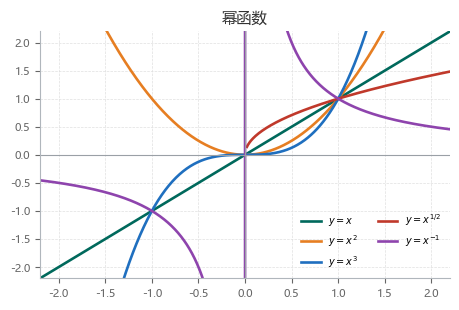
\includegraphics[width=0.52\textwidth]{figs/func_power.png}\hfill
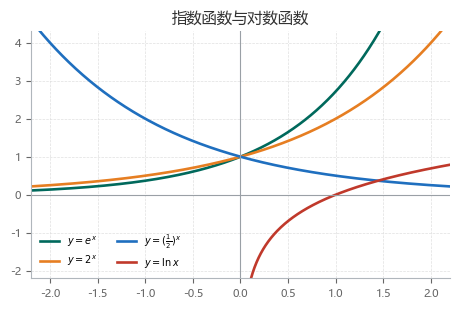
\includegraphics[width=0.46\textwidth]{figs/func_explog.png}
\end{center}
\begin{center}
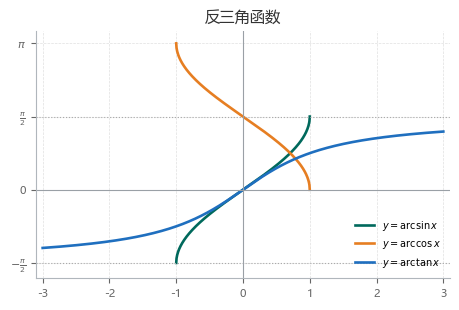
\includegraphics[width=0.52\textwidth]{figs/func_trig_inv.png}
\end{center}
\end{formbox}

\hd{常用初等恒等式与因式分解}
\begin{formbox}
\renewcommand{\arraystretch}{1.6}
\[
\begin{aligned}
(a+b)^{2}&=a^{2}+2ab+b^{2}, & (a-b)^{2}&=a^{2}-2ab+b^{2},\\[2pt]
(a+b)^{3}&=a^{3}+3a^{2}b+3ab^{2}+b^{3}, & (a-b)^{3}&=a^{3}-3a^{2}b+3ab^{2}-b^{3},\\[2pt]
a^{3}+b^{3}&=(a+b)(a^{2}-ab+b^{2}), & a^{3}-b^{3}&=(a-b)(a^{2}+ab+b^{2}),\\[2pt]
a^{n}-b^{n}&=(a-b)\sum_{i=0}^{n-1}a^{\,n-1-i}b^{i}.
\end{aligned}
\]
\[
\text{求根公式：}\quad x=\frac{-b\pm\sqrt{b^{2}-4ac}}{2a},
\qquad
\text{韦达定理：}\quad x_{1}+x_{2}=-\frac ba,\ \ x_{1}x_{2}=\frac ca
\]
\end{formbox}

\hd{基本不等式与均值不等式}
\begin{formbox}
\[
\bx{\bigl||a|-|b|\bigr|\le|a\pm b|\le|a|+|b|},
\qquad
\bx{2ab\le a^{2}+b^{2}}\qquad(a,b\in\mathbb R)
\]
\[
\bx{\frac{2}{\frac1a+\frac1b}\le\sqrt{ab}\le\frac{a+b}{2}\le\sqrt{\frac{a^{2}+b^{2}}{2}}}
\qquad(a,b>0)
\]
\[
ab\le\Bigl(\frac{a+b}{2}\Bigr)^{2}\le\frac{a^{2}+b^{2}}{2}\ \ (a,b>0),
\qquad
\frac{(a+b)^{2}}{2}\le a^{2}+b^{2}
\]
\end{formbox}

\begin{formbox}
\[
\frac{n}{\displaystyle\sum_{i=1}^{n}\frac1{a_{i}}}\le\sqrt[n]{\prod_{i=1}^{n}a_{i}}
\le\frac{\displaystyle\sum_{i=1}^{n}a_{i}}{n}
\le\sqrt{\frac{\displaystyle\sum_{i=1}^{n}a_{i}^{2}}{n}}
\qquad(a_{i}>0)
\]
\[
\bx{\Bigl(\sum_{i=1}^{n}a_{i}^{2}\Bigr)\Bigl(\sum_{i=1}^{n}b_{i}^{2}\Bigr)
\ge\Bigl(\sum_{i=1}^{n}a_{i}b_{i}\Bigr)^{2}}\qquad\text{（柯西不等式）}
\]
\[
a^{2}+b^{2}+c^{2}\ge ab+bc+ca,\qquad
a^{3}+b^{3}+c^{3}\ge3abc\ \ (a,b,c>0)
\]
\[
ab>0\Rightarrow\frac ab+\frac ba\ge2;\qquad
ab<0\Rightarrow\frac ab+\frac ba\le-2
\]
\[
\frac ba<\frac{b+m}{a+m}<1\qquad(a>b>0,\ m>0)
\]
\end{formbox}

\hd{常用函数不等式}
\begin{formbox}
\[
\bx{\sin x<x<\tan x}\quad\Bigl(0<x<\tfrac{\pi}{2}\Bigr),\qquad
\sin x<x\quad(x>0)
\]
\[
\arcsin x\ge x\quad(0\le x\le1),\qquad
\arctan x\le x\quad(x\ge0)
\]
\[
e^{x}\ge x+1,\qquad
\frac{x}{1+x}\le\ln(1+x)\le x\quad(x>-1),\qquad
\ln x\le x-1\quad(x>0)
\]
\end{formbox}

\hd{三角函数公式（同角、和差、倍半角）}
\begin{formbox}
\renewcommand{\arraystretch}{1.7}
\[
\begin{aligned}
\sin^{2}\alpha+\cos^{2}\alpha&=1, & 1+\tan^{2}\alpha&=\sec^{2}\alpha, & 1+\cot^{2}\alpha&=\csc^{2}\alpha,\\[2pt]
\sin(\alpha\pm\beta)&=\sin\alpha\cos\beta\pm\cos\alpha\sin\beta,
& \cos(\alpha\pm\beta)&=\cos\alpha\cos\beta\mp\sin\alpha\sin\beta,\\[2pt]
\tan(\alpha\pm\beta)&=\frac{\tan\alpha\pm\tan\beta}{1\mp\tan\alpha\tan\beta}.
\end{aligned}
\]
\[
\begin{aligned}
\sin 2\alpha&=2\sin\alpha\cos\alpha,
&\cos 2\alpha=\cos^{2}\alpha-\sin^{2}\alpha&=2\cos^{2}\alpha-1=1-2\sin^{2}\alpha,\\[2pt]
\tan 2\alpha&=\frac{2\tan\alpha}{1-\tan^{2}\alpha},
& \sin^{2}\alpha&=\frac{1-\cos 2\alpha}{2},\quad
\cos^{2}\alpha=\frac{1+\cos 2\alpha}{2}.
\end{aligned}
\]
\[
\begin{aligned}
\text{万能代换：}\quad
\sin\alpha&=\frac{2t}{1+t^{2}}, &
\cos\alpha&=\frac{1-t^{2}}{1+t^{2}}, &
\tan\alpha&=\frac{2t}{1-t^{2}},\qquad t=\tan\frac{\alpha}{2},\\[3pt]
\text{辅助角：}\quad
a\sin x+b\cos x&=\sqrt{a^{2}+b^{2}}\sin(x+\varphi),
&\tan\varphi&=\frac ba .
\end{aligned}
\]
\end{formbox}

\hd{和差化积与积化和差}
\begin{formbox}
\renewcommand{\arraystretch}{1.7}
\[
\begin{aligned}
\sin\alpha+\sin\beta&=2\sin\frac{\alpha+\beta}{2}\cos\frac{\alpha-\beta}{2},
& \sin\alpha-\sin\beta&=2\cos\frac{\alpha+\beta}{2}\sin\frac{\alpha-\beta}{2},\\[3pt]
\cos\alpha+\cos\beta&=2\cos\frac{\alpha+\beta}{2}\cos\frac{\alpha-\beta}{2},
& \cos\alpha-\cos\beta&=-2\sin\frac{\alpha+\beta}{2}\sin\frac{\alpha-\beta}{2}.
\end{aligned}
\]
\[
\begin{aligned}
\sin\alpha\cos\beta&=\tfrac12\bigl[\sin(\alpha+\beta)+\sin(\alpha-\beta)\bigr],
& \cos\alpha\sin\beta&=\tfrac12\bigl[\sin(\alpha+\beta)-\sin(\alpha-\beta)\bigr],\\[3pt]
\cos\alpha\cos\beta&=\tfrac12\bigl[\cos(\alpha+\beta)+\cos(\alpha-\beta)\bigr],
& \sin\alpha\sin\beta&=-\tfrac12\bigl[\cos(\alpha+\beta)-\cos(\alpha-\beta)\bigr].
\end{aligned}
\]
\end{formbox}

\hd{两个重要极限与常用极限}
\begin{formbox}
\[
\bx{\lim_{x\to0}\frac{\sin x}{x}=1},
\qquad
\bx{\lim_{x\to\infty}\Bigl(1+\frac1x\Bigr)^{x}=e},
\qquad
\bx{\lim_{x\to0}(1+x)^{\frac1x}=e}
\]
\[
\lim_{\varphi(x)\to0}\frac{\sin\varphi(x)}{\varphi(x)}=1,
\qquad
\lim_{\varphi(x)\to\infty}\Bigl(1+\frac1{\varphi(x)}\Bigr)^{\varphi(x)}=e,
\qquad
\lim_{\varphi(x)\to0}\bigl(1+\varphi(x)\bigr)^{\frac1{\varphi(x)}}=e
\]
\end{formbox}

\hd{等价无穷小（$x\to0$）}
\begin{formbox}
\renewcommand{\arraystretch}{1.6}
\[
\begin{aligned}
&\sin x\sim x, & \tan x\sim x, & \arcsin x\sim x, & \arctan x\sim x,\\[3pt]
&\ln(1+x)\sim x, & e^{x}-1\sim x, & a^{x}-1\sim x\ln a, & \log_a(1+x)\sim\frac{x}{\ln a},\\[3pt]
&(1+x)^{\alpha}-1\sim\alpha x, & 1-\cos x\sim\frac{x^{2}}{2}.
\end{aligned}
\]
\[
\begin{aligned}
&x-\sin x\sim\frac{x^{3}}{6}, & \arcsin x-x\sim\frac{x^{3}}{6},
& \tan x-x\sim\frac{x^{3}}{3}, & x-\arctan x\sim\frac{x^{3}}{3},\\[3pt]
&\tan x-\sin x\sim\frac{x^{3}}{2}.
\end{aligned}
\]
\end{formbox}

\hd{无穷小的比较}
\begin{formbox}
设 $\alpha,\beta$ 为同一极限过程的无穷小，且 $\beta\ne0$：
\[
\lim\frac{\alpha}{\beta}=0\ \Rightarrow\ \alpha=o(\beta)\ \text{（高阶）},\qquad
\lim\frac{\alpha}{\beta}=\infty\ \Rightarrow\ \text{低阶}
\]
\[
\lim\frac{\alpha}{\beta}=c\ne0\ \Rightarrow\ \text{同阶},\qquad
\lim\frac{\alpha}{\beta}=1\ \Rightarrow\ \alpha\sim\beta\ \text{（等价）}
\]
\end{formbox}

\hd{极限运算法则与存在准则}
\begin{formbox}
\[
\text{若}\ \lim f(x)=A,\ \lim g(x)=B\ \text{存在，则}\qquad
\lim\bigl[f(x)\pm g(x)\bigr]=A\pm B
\]
\[
\lim\bigl[f(x)g(x)\bigr]=AB,\qquad
\lim\frac{f(x)}{g(x)}=\frac{A}{B}\ \ (B\ne0)
\]
\[
\bx{\text{夹逼准则：}\quad g(x)\le f(x)\le h(x),\ \lim g=\lim h=A\ \Rightarrow\ \lim f=A}
\]
\[
\bx{\text{单调有界准则：}\quad \text{单调有界数列必有极限}}
\]
\end{formbox}

\hd{连续性}
\begin{formbox}
\[
f\ \text{在}\ x_{0}\ \text{连续}\iff\lim_{x\to x_{0}}f(x)=f(x_{0})
\iff\lim_{x\to x_{0}^{-}}f(x)=\lim_{x\to x_{0}^{+}}f(x)=f(x_{0})
\]
间断点分类：第一类（左右极限均存在：可去型、跳跃型）；第二类（至少一侧极限不存在：无穷、振荡等）。

闭区间上连续函数 $f\in C[a,b]$ 的性质：
\[
\bx{\text{零点定理：}\ f(a)f(b)<0\Rightarrow\exists\,\xi\in(a,b),\ f(\xi)=0}
\]
\[
\bx{\text{介值定理：}\ f\ \text{可取到}\ f(a)\ \text{与}\ f(b)\ \text{之间的任何值}}
\]
\[
\bx{\text{最值定理：}\ f\ \text{在}\ [a,b]\ \text{上有界，且取得最大值与最小值}}
\]
\end{formbox}
\end{secbox}

% ============================================================
\begin{secbox}[二、一元函数微分学]

\hd{导数与微分}
\begin{formbox}
\[
f'(x_{0})=\lim_{\Delta x\to0}\frac{f(x_{0}+\Delta x)-f(x_{0})}{\Delta x}
=\lim_{x\to x_{0}}\frac{f(x)-f(x_{0})}{x-x_{0}},
\qquad
\mathrm dy=f'(x)\,\mathrm dx
\]
\bx{\text{可导}\iff\text{可微}}（一元函数）；可导必连续，连续不一定可导。
\end{formbox}

\hd{基本求导公式}
\begin{formbox}
\renewcommand{\arraystretch}{1.6}
\[
\begin{array}{llll}
(C)'=0 & (x^{\alpha})'=\alpha x^{\alpha-1} & (a^{x})'=a^{x}\ln a & (e^{x})'=e^{x}\\[4pt]
(\log_a x)'=\dfrac1{x\ln a} & (\ln x)'=\dfrac1x & (\sin x)'=\cos x & (\cos x)'=-\sin x\\[4pt]
(\tan x)'=\sec^{2}x & (\cot x)'=-\csc^{2}x & (\sec x)'=\sec x\tan x & (\csc x)'=-\csc x\cot x\\[4pt]
(\arcsin x)'=\dfrac1{\sqrt{1-x^{2}}} & (\arccos x)'=-\dfrac1{\sqrt{1-x^{2}}}
& (\arctan x)'=\dfrac1{1+x^{2}} & (\operatorname{arccot} x)'=-\dfrac1{1+x^{2}}
\end{array}
\]
\end{formbox}

\hd{求导法则}
\begin{formbox}
\renewcommand{\arraystretch}{1.6}
\[
\begin{aligned}
(u\pm v)'&=u'\pm v', & (uv)'&=u'v+uv', & \Bigl(\frac uv\Bigr)'&=\frac{u'v-uv'}{v^{2}},\\[3pt]
\text{复合：}\ \frac{\mathrm dy}{\mathrm dx}&=\frac{\mathrm dy}{\mathrm du}\cdot\frac{\mathrm du}{\mathrm dx},
& \text{反函数：}\ \frac{\mathrm dx}{\mathrm dy}&=\frac1{\,\mathrm dy/\mathrm dx\,}.
\end{aligned}
\]
\begin{tabular}{@{}p{4.6cm}p{11.4cm}@{}}
隐函数 $F(x,y)=0$ & 方程两边对 $x$ 求导（把 $y$ 当 $x$ 的函数），解出 $y'=-\dfrac{F_x}{F_y}$\\[4pt]
参数方程 $\begin{cases}x=\varphi(t)\\ y=\psi(t)\end{cases}$ &
  $\dfrac{\mathrm dy}{\mathrm dx}=\dfrac{\psi'(t)}{\varphi'(t)}$，
  $\dfrac{\mathrm d^{2}y}{\mathrm dx^{2}}=\dfrac{\mathrm d}{\mathrm dt}\Bigl(\dfrac{\psi'}{\varphi'}\Bigr)\cdot\dfrac1{\varphi'(t)}$\\[4pt]
对数求导 & $y=u(x)^{v(x)}$ 取 $\ln y=v\ln u$ 后两边求导
\end{tabular}
\end{formbox}

\hd{高阶导数与莱布尼茨公式}
\begin{formbox}
\[
\bx{(uv)^{(n)}=\sum_{i=0}^{n}C_{n}^{i}u^{(n-i)}v^{(i)}}
\]
\[
\renewcommand{\arraystretch}{1.6}
\begin{array}{ll}
(e^{ax})^{(n)}=a^{n}e^{ax} & \bigl(\ln(1+x)\bigr)^{(n)}=\dfrac{(-1)^{n-1}(n-1)!}{(1+x)^{n}}\\[10pt]
(\sin ax)^{(n)}=a^{n}\sin\Bigl(ax+\dfrac{n\pi}{2}\Bigr)
& \bigl((1+x)^{\alpha}\bigr)^{(n)}=\alpha(\alpha-1)\cdots(\alpha-n+1)(1+x)^{\alpha-n}\\[10pt]
(\cos ax)^{(n)}=a^{n}\cos\Bigl(ax+\dfrac{n\pi}{2}\Bigr)
& \bigl((1+x)^{n}\bigr)^{(n)}=n!,\qquad \bigl((1+x)^{n}\bigr)^{(n+j)}=0
\end{array}
\]
\end{formbox}

\hd{微分中值定理}
\begin{formbox}
\[
\bx{\text{罗尔：}\ f\in C[a,b],\ f\ \text{在}\ (a,b)\ \text{可导},\ f(a)=f(b)
\ \Rightarrow\ \exists\,\xi\in(a,b),\ f'(\xi)=0}
\]
\[
\bx{\text{拉格朗日：}\ f\in C[a,b],\ \text{可导}\ \Rightarrow\ \exists\,\xi\in(a,b),\ 
f'(\xi)=\frac{f(b)-f(a)}{b-a}}
\]
\[
\bx{\text{柯西：}\ \exists\,\xi\in(a,b),\ 
\frac{f'(\xi)}{g'(\xi)}=\frac{f(b)-f(a)}{g(b)-g(a)}}\qquad(g'\ne0)
\]
\end{formbox}

\hd{泰勒公式与麦克劳林公式}
\begin{formbox}
\[
f(x)=\sum_{k=0}^{n}\frac{f^{(k)}(x_{0})}{k!}(x-x_{0})^{k}+R_{n}(x),
\qquad
R_{n}(x)=\frac{f^{(n+1)}(\xi)}{(n+1)!}(x-x_{0})^{n+1}\ \text{（拉格朗日余项）}
\]
\[
x_{0}=0\ \text{时：}\quad f(x)=\sum_{k=0}^{n}\frac{f^{(k)}(0)}{k!}x^{k}+o(x^{n})\ \text{（皮亚诺余项）}
\]
\end{formbox}

\hd{麦克劳林展开（含收敛域）}
\begin{formbox}
\[
\renewcommand{\arraystretch}{1.55}
\begin{array}{lll}
e^{x}=\displaystyle\sum_{n=0}^{\infty}\frac{x^{n}}{n!}=1+x+\dfrac{x^{2}}{2!}+\dfrac{x^{3}}{3!}+o(x^{3})
  &\cond{x\in(-\infty,+\infty)}\\[8pt]
\sin x=\displaystyle\sum_{n=0}^{\infty}\frac{(-1)^{n}}{(2n+1)!}x^{2n+1}
  =x-\dfrac{x^{3}}{3!}+\dfrac{x^{5}}{5!}+o(x^{5})
  &\cond{x\in(-\infty,+\infty)}\\[8pt]
\cos x=\displaystyle\sum_{n=0}^{\infty}\frac{(-1)^{n}}{(2n)!}x^{2n}
  =1-\dfrac{x^{2}}{2!}+\dfrac{x^{4}}{4!}+o(x^{4})
  &\cond{x\in(-\infty,+\infty)}\\[8pt]
\ln(1+x)=\displaystyle\sum_{n=1}^{\infty}\frac{(-1)^{n-1}}{n}x^{n}
  =x-\dfrac{x^{2}}{2}+\dfrac{x^{3}}{3}+o(x^{3})
  &\cond{x\in(-1,1]}\\[8pt]
(1+x)^{\alpha}=1+\alpha x+\dfrac{\alpha(\alpha-1)}{2!}x^{2}+\dfrac{\alpha(\alpha-1)(\alpha-2)}{3!}x^{3}+o(x^{3})
  &\cond{x\in(-1,1)}\\[8pt]
\dfrac{1}{1-x}=\displaystyle\sum_{n=0}^{\infty}x^{n}=1+x+x^{2}+x^{3}+o(x^{3})
  &\cond{x\in(-1,1)}\\[8pt]
\dfrac{1}{1+x}=\displaystyle\sum_{n=0}^{\infty}(-1)^{n}x^{n}=1-x+x^{2}-x^{3}+o(x^{3})
  &\cond{x\in(-1,1)}\\[8pt]
\tan x=x+\dfrac{x^{3}}{3}+\dfrac{2x^{5}}{15}+o(x^{5})
  &\cond{x\in\left(-\tfrac{\pi}{2},\tfrac{\pi}{2}\right)}\\[8pt]
\arcsin x=x+\dfrac{x^{3}}{6}+\dfrac{3x^{5}}{40}+o(x^{5})
  &\cond{x\in[-1,1]}\\[8pt]
\arctan x=x-\dfrac{x^{3}}{3}+\dfrac{x^{5}}{5}+o(x^{5})
  &\cond{x\in[-1,1]}
\end{array}
\]
\end{formbox}

\hd{洛必达法则}
\begin{formbox}
\[
\bx{\lim\frac{f(x)}{g(x)}=\lim\frac{f'(x)}{g'(x)}}
\qquad\text{用于}\ \frac00\ \text{或}\ \frac{\infty}{\infty}\ \text{型}
\]
\textbf{注意：}使用前必须验证是 $\frac00$ 或 $\frac{\infty}{\infty}$ 型；其它未定式 $0\cdot\infty,\ \infty-\infty,\ 1^{\infty},\ 0^{0},\ \infty^{0}$ 先化归为 $\frac00$ 或 $\frac{\infty}{\infty}$ 型。
\end{formbox}

\hd{函数性态（单调、极值、凹凸、拐点、渐近线）}
\begin{formbox}
\[
\begin{aligned}
\text{单调性：}\ &f'(x)>0\Rightarrow f\ \text{增};\quad f'(x)<0\Rightarrow f\ \text{减}.\\[3pt]
\text{极值：}\ &f'(x_{0})=0\ \text{或不存在（驻点/不可导点），两侧判号}:\\[3pt]
&f'\ \text{左正右负}\Rightarrow\text{极大};\quad f'\ \text{左负右正}\Rightarrow\text{极小}.
\end{aligned}
\]
\[
\bx{f''(x_{0})>0\Rightarrow x_{0}\ \text{为极小值点}},\qquad
\bx{f''(x_{0})<0\Rightarrow x_{0}\ \text{为极大值点}}
\]
\[
\begin{aligned}
\text{凹凸：}\ f''(x)>0\Rightarrow\text{凹（上凹）};\quad f''(x)<0\Rightarrow\text{凸}.
\quad \text{拐点：}\ f''(x_{0})=0\ \text{且两侧}\ f''\ \text{变号}.
\end{aligned}
\]
\[
\begin{aligned}
\text{水平渐近线：}\ &y=b,\ \lim_{x\to\infty}f(x)=b\\
\text{铅直渐近线：}\ &x=x_{0},\ \lim_{x\to x_{0}}f(x)=\infty\\
\text{斜渐近线：}\ &y=kx+b,\quad k=\lim_{x\to\infty}\frac{f(x)}{x},\ \ b=\lim_{x\to\infty}\bigl[f(x)-kx\bigr]
\end{aligned}
\]
\end{formbox}

\hd{经济应用（边际、弹性、连续复利）}
\begin{formbox}
\[
\text{边际成本：}\ MC=C'(q),\qquad
\text{边际收益：}\ MR=R'(q),\qquad
\text{边际利润：}\ L'(q)=R'(q)-C'(q)
\]
\[
\bx{\text{需求的价格弹性：}\ \eta=-\frac{P}{Q}\,\frac{\mathrm dQ}{\mathrm dP}=-\frac{P\,Q'(P)}{Q(P)}}
\]
\[
\bx{\text{连续复利：}\ A=Pe^{rt}}
\qquad
\text{（本金}\ P\ \text{、年利率}\ r\ \text{、连续计息}\ t\ \text{年后的本利和）}
\]
\end{formbox}
\end{secbox}

% ============================================================
\begin{secbox}[三、一元函数积分学]

\hd{基本积分公式}
\begin{formbox}
\renewcommand{\arraystretch}{1.7}
\[
\begin{array}{ll}
\displaystyle\int x^{a}\,\mathrm dx=\frac{x^{a+1}}{a+1}+C\ \ (a\ne-1)
& \displaystyle\int\frac1x\,\mathrm dx=\ln|x|+C\\[5pt]
\displaystyle\int a^{x}\,\mathrm dx=\frac{a^{x}}{\ln a}+C\ \ (a>0,a\ne1)
& \displaystyle\int e^{x}\,\mathrm dx=e^{x}+C\\[5pt]
\displaystyle\int\sin x\,\mathrm dx=-\cos x+C
& \displaystyle\int\cos x\,\mathrm dx=\sin x+C\\[5pt]
\displaystyle\int\tan x\,\mathrm dx=-\ln|\cos x|+C
& \displaystyle\int\cot x\,\mathrm dx=\ln|\sin x|+C\\[5pt]
\displaystyle\int\sec x\,\mathrm dx=\ln|\sec x+\tan x|+C
& \displaystyle\int\csc x\,\mathrm dx=\ln|\csc x-\cot x|+C\\[5pt]
\displaystyle\int\sec^{2}x\,\mathrm dx=\tan x+C
& \displaystyle\int\csc^{2}x\,\mathrm dx=-\cot x+C
\end{array}
\]
\[
\begin{array}{ll}
\displaystyle\int\frac1{1+x^{2}}\,\mathrm dx=\arctan x+C
& \displaystyle\int\frac1{\sqrt{1-x^{2}}}\,\mathrm dx=\arcsin x+C\\[6pt]
\displaystyle\int\frac1{a^{2}+x^{2}}\,\mathrm dx=\frac1a\arctan\frac{x}{a}+C
& \displaystyle\int\frac1{a^{2}-x^{2}}\,\mathrm dx=\frac1{2a}\ln\left|\frac{a+x}{a-x}\right|+C\\[6pt]
\displaystyle\int\frac1{\sqrt{a^{2}-x^{2}}}\,\mathrm dx=\arcsin\frac{x}{a}+C
& \displaystyle\int\frac1{\sqrt{x^{2}\pm a^{2}}}\,\mathrm dx=\ln\left|x+\sqrt{x^{2}\pm a^{2}}\right|+C\\[6pt]
\displaystyle\int\sqrt{a^{2}-x^{2}}\,\mathrm dx=\frac{x}{2}\sqrt{a^{2}-x^{2}}+\frac{a^{2}}{2}\arcsin\frac{x}{a}+C
& \\[8pt]
\displaystyle\int\sqrt{x^{2}\pm a^{2}}\,\mathrm dx=\frac{x}{2}\sqrt{x^{2}\pm a^{2}}\pm\frac{a^{2}}{2}\ln\left|x+\sqrt{x^{2}\pm a^{2}}\right|+C
&
\end{array}
\]
\end{formbox}

\hd{换元积分与分部积分}
\begin{formbox}
\[
\bx{\text{第一换元（凑微分）：}\ \int f\bigl[\varphi(x)\bigr]\varphi'(x)\,\mathrm dx=\int f(u)\,\mathrm du}
\]
\[
\bx{\text{第二换元：}\ \int f(x)\,\mathrm dx\ \xrightarrow{\ x=\psi(t)\ }\
\int f\bigl[\psi(t)\bigr]\psi'(t)\,\mathrm dt}
\]
\[
\bx{\text{分部积分：}\ \int u\,\mathrm dv=uv-\int v\,\mathrm du}
\qquad\text{（反对幂指三，谁靠后谁作 }\mathrm dv\text{）}
\]
\[
\text{三角代换：}\quad
\sqrt{a^{2}-x^{2}}\xrightarrow{\,x=a\sin t\,},\ \
\sqrt{x^{2}+a^{2}}\xrightarrow{\,x=a\tan t\,},\ \
\sqrt{x^{2}-a^{2}}\xrightarrow{\,x=a\sec t\,}
\]
\[
\text{万能代换：}\ t=\tan\frac{x}{2},\quad
\sin x=\frac{2t}{1+t^{2}},\quad\cos x=\frac{1-t^{2}}{1+t^{2}},\quad
\mathrm dx=\frac{2}{1+t^{2}}\,\mathrm dt
\]
\end{formbox}

\hd{有理函数与常见特殊积分}
\begin{formbox}
\[
\int\frac{P(x)}{Q(x)}\,\mathrm dx:\ \text{先化为真分式，分母因式分解，拆成部分分式再积分}
\]
\[
\int R\!\left(x,\sqrt{\frac{ax+b}{cx+d}}\right)\mathrm dx
\ \overset{\sqrt{\frac{ax+b}{cx+d}}=t}{=}\
\int R\!\left(\frac{dt^{2}-b}{a-ct^{2}},\,t\right)\frac{2(ad-bc)t}{(a-ct^{2})^{2}}\,\mathrm dt
\qquad\cond{ad-bc\ne0}
\]
\[
\int x^{n}e^{x}\,\mathrm dx=e^{x}\sum_{i=0}^{n}(-1)^{i}\bigl(x^{n}\bigr)^{(i)}+C,
\qquad
\int_{0}^{+\infty}x^{n}e^{-x}\,\mathrm dx=n!=\Gamma(n+1)
\]
\[
\int_{-\infty}^{+\infty}e^{-x^{2}}\,\mathrm dx=\sqrt{\pi}
\]
\end{formbox}

\hd{定积分性质}
\begin{formbox}
\[
\begin{aligned}
&\int_{a}^{b}\bigl[\alpha f(x)+\beta g(x)\bigr]\mathrm dx=\alpha\int_{a}^{b}f+\beta\int_{a}^{b}g,
\quad
\int_{a}^{b}f=\int_{a}^{c}f+\int_{c}^{b}f,\\[3pt]
&f(x)\ge0\ \Rightarrow\ \int_{a}^{b}f(x)\mathrm dx\ge0,
\qquad
\Bigl|\int_{a}^{b}f\,\mathrm dx\Bigr|\le\int_{a}^{b}|f|\,\mathrm dx.
\end{aligned}
\]
\[
\bx{\text{积分中值定理：}\ \exists\,\xi\in[a,b],\ \int_{a}^{b}f(x)\mathrm dx=f(\xi)(b-a)}
\]
\[
\begin{aligned}
\text{奇偶性：}&
\int_{-a}^{a}f=\begin{cases}2\displaystyle\int_{0}^{a}f, & f\ \text{为偶}\\[4pt] 0, & f\ \text{为奇}\end{cases}\\
\text{周期性：}&
\int_{a}^{a+T}f(x)\,\mathrm dx=\int_{0}^{T}f(x)\,\mathrm dx.
\end{aligned}
\]
\end{formbox}

\hd{变上限积分（微积分基本定理）}
\begin{formbox}
\[
\bx{\Phi(x)=\int_{a}^{x}f(t)\,\mathrm dt\ \Rightarrow\ \Phi'(x)=f(x)}
\]
\[
\bx{\frac{\mathrm d}{\mathrm dx}\int_{a}^{\varphi(x)}f(t)\,\mathrm dt=f\bigl[\varphi(x)\bigr]\varphi'(x)}
\]
\[
\frac{\mathrm d}{\mathrm dx}\int_{\psi(x)}^{\varphi(x)}f(t)\,\mathrm dt
=f\bigl[\varphi(x)\bigr]\varphi'(x)-f\bigl[\psi(x)\bigr]\psi'(x)
\]
\[
\bx{\text{牛—莱公式：}\ \int_{a}^{b}f(x)\,\mathrm dx=F(b)-F(a),\quad F'=f}
\]
\end{formbox}

\hd{反常积分}
\begin{formbox}
\[
\int_{a}^{+\infty}f(x)\mathrm dx=\lim_{b\to+\infty}\int_{a}^{b}f(x)\mathrm dx,
\qquad
\int_{a}^{b}f(x)\mathrm dx=\lim_{\varepsilon\to0^{+}}\int_{a+\varepsilon}^{b}f(x)\mathrm dx\ \text{（瑕积分）}
\]
\[
\bx{\int_{1}^{+\infty}\frac1{x^{p}}\,\mathrm dx\ \text{收敛}\iff p>1},
\qquad
\bx{\int_{0}^{1}\frac1{x^{p}}\,\mathrm dx\ \text{收敛}\iff p<1}
\]
\end{formbox}

\hd{定积分应用（面积、体积、弧长）}
\begin{formbox}
\[
\text{平面面积：}\quad
A=\int_{a}^{b}\bigl[f_{\text{上}}(x)-f_{\text{下}}(x)\bigr]\mathrm dx,
\qquad
A=\frac12\int_{\alpha}^{\beta}r^{2}(\theta)\,\mathrm d\theta
\]
\[
\text{旋转体体积（绕 }x\text{ 轴）：}\quad
V_{x}=\pi\int_{a}^{b}f^{2}(x)\,\mathrm dx,
\qquad
\text{绕 }y\text{ 轴（壳法）：}\quad
V_{y}=2\pi\int_{a}^{b}xf(x)\,\mathrm dx
\]
\[
\text{弧长：}\quad
s=\int_{a}^{b}\sqrt{1+(y')^{2}}\,\mathrm dx,
\quad
s=\int_{\alpha}^{\beta}\sqrt{(x')^{2}+(y')^{2}}\,\mathrm dt,
\quad
s=\int_{\alpha}^{\beta}\sqrt{r^{2}+(r')^{2}}\,\mathrm d\theta
\]
\end{formbox}

\hd{华里士（Wallis）公式}
\begin{formbox}
\[
\bx{\int_{0}^{\frac{\pi}{2}}\sin^{n}x\,\mathrm dx=\int_{0}^{\frac{\pi}{2}}\cos^{n}x\,\mathrm dx
=\begin{cases}
\dfrac{n-1}{n}\cdot\dfrac{n-3}{n-2}\cdots\dfrac12\cdot\dfrac{\pi}{2}, & n\ \text{为偶}\\[8pt]
\dfrac{n-1}{n}\cdot\dfrac{n-3}{n-2}\cdots\dfrac23\cdot 1, & n\ \text{为奇}
\end{cases}}
\]
\[
\int_{0}^{\pi}\sin^{n}x\,\mathrm dx=2\int_{0}^{\frac{\pi}{2}}\sin^{n}x\,\mathrm dx,
\qquad
\int_{0}^{2\pi}\sin^{n}x\,\mathrm dx=
\begin{cases}
4\displaystyle\int_{0}^{\frac{\pi}{2}}\sin^{n}x, & n\ \text{为偶}\\[6pt]
0, & n\ \text{为奇}
\end{cases}
\]
\end{formbox}
\end{secbox}

% ============================================================
\begin{secbox}[四、多元函数微积分学]

\hd{偏导数与全微分}
\begin{formbox}
\[
f_{x}(x_{0},y_{0})=\lim_{\Delta x\to0}\frac{f(x_{0}+\Delta x,y_{0})-f(x_{0},y_{0})}{\Delta x}
\]
\[
\bx{\mathrm dz=\frac{\partial z}{\partial x}\mathrm dx+\frac{\partial z}{\partial y}\mathrm dy}
\qquad
\text{偏导连续}\Rightarrow\text{可微}\Rightarrow\text{可导、连续}
\]
\[
\text{可微}\iff
\frac{\Delta z-f_{x}\Delta x-f_{y}\Delta y}{\sqrt{(\Delta x)^{2}+(\Delta y)^{2}}}\to0
\]
\end{formbox}

\hd{复合函数与隐函数求导}
\begin{formbox}
\[
z=f(u,v),\ u=u(x,y),\ v=v(x,y):
\quad
\frac{\partial z}{\partial x}=\frac{\partial f}{\partial u}\frac{\partial u}{\partial x}
+\frac{\partial f}{\partial v}\frac{\partial v}{\partial x}
\]
\[
F(x,y)=0:\ \frac{\mathrm dy}{\mathrm dx}=-\frac{F_x}{F_y},
\qquad
F(x,y,z)=0:\ 
\frac{\partial z}{\partial x}=-\frac{F_x}{F_z},\ \
\frac{\partial z}{\partial y}=-\frac{F_y}{F_z}
\]
\end{formbox}

\hd{多元无条件极值}
\begin{formbox}
设 $z=f(x,y)$ 在驻点（$f_x=f_y=0$）处令
$f''_{xx}=A,\ f''_{xy}=B,\ f''_{yy}=C$：
\[
\bx{\begin{cases}
AC-B^{2}>0, & A>0\ \text{极小};\ A<0\ \text{极大}\\[3pt]
AC-B^{2}<0, & \text{非极值}\\[3pt]
AC-B^{2}=0, & \text{无法判断}
\end{cases}}
\]
\end{formbox}

\hd{条件极值（拉格朗日乘数法）}
\begin{formbox}
求 $z=f(x,y)$ 在条件 $\varphi(x,y)=0$ 下的极值：
\[
\bx{L(x,y,\lambda)=f(x,y)+\lambda\varphi(x,y)},
\qquad
\text{令}\quad
\begin{cases}
L_{x}=0\\ L_{y}=0\\ L_{\lambda}=\varphi(x,y)=0
\end{cases}
\]
\end{formbox}

\hd{二重积分}
\begin{formbox}
\[
\iint_{D}f(x,y)\,\mathrm d\sigma=\int_{a}^{b}\mathrm dx\int_{y_{1}(x)}^{y_{2}(x)}f(x,y)\,\mathrm dy
\]
\[
\bx{\text{极坐标：}\quad x=r\cos\theta,\ y=r\sin\theta,\ \mathrm d\sigma=r\,\mathrm dr\,\mathrm d\theta}
\]
\[
\begin{aligned}
\text{对称性：}&\ D\ \text{关于}\ y\ \text{轴对称，}\ f\ \text{为}\ x\ \text{的奇函数}\Rightarrow\iint_{D}f=0;\\
&\ f\ \text{为}\ x\ \text{的偶函数}\Rightarrow\iint_{D}f=2\iint_{D_{\text{右}}}f.
\end{aligned}
\]
\[
\text{轮换对称性：若}\ D\ \text{关于}\ x=y\ \text{对称},\ \text{则}\ \iint_{D}f(x,y)\,\mathrm d\sigma=\iint_{D}f(y,x)\,\mathrm d\sigma
\]
\end{formbox}
\end{secbox}

% ============================================================
\begin{secbox}[五、无穷级数]

\hd{常用数列与求和公式}
\begin{formbox}
\[
a_{n}=a_{1}+(n-1)d\quad\Rightarrow\quad
S_{n}=\frac{n}{2}(a_{1}+a_{n})=na_{1}+\frac{n(n-1)}{2}d
\]
\[
a_{n}=a_{1}q^{\,n-1}\ (q\ne1)\quad\Rightarrow\quad
S_{n}=\frac{a_{1}(1-q^{n})}{1-q}=\frac{a_{1}-a_{n}q}{1-q}
\]
\[
\sum_{k=1}^{n}k=\frac{n(n+1)}{2},\qquad
\sum_{k=1}^{n}k^{2}=\frac{n(n+1)(2n+1)}{6},\qquad
\sum_{k=1}^{n}k^{3}=\Bigl[\frac{n(n+1)}{2}\Bigr]^{2}
\]
\end{formbox}

\hd{常数项级数敛散性判据}
\begin{formbox}
\[
\bx{\sum u_{n}\ \text{收敛}\ \Rightarrow\ \lim_{n\to\infty}u_{n}=0}\qquad
\text{（反之不成立，仅作否定判别）}
\]
\[
\begin{aligned}
\text{几何级数：}\ &\sum_{n=0}^{\infty}q^{n}\ \text{收敛}\iff|q|<1,\ \text{和为}\ \frac1{1-q}\\
\text{调和级数：}\ &\sum_{n=1}^{\infty}\frac1n\ \text{发散};
\qquad
\text{p 级数：}\ \sum_{n=1}^{\infty}\frac1{n^{p}}\ \text{收敛}\iff p>1
\end{aligned}
\]
\end{formbox}

\begin{formbox}
\[
\text{正项级数判据}:
\begin{cases}
\text{比较法：}\ u_{n}\le v_{n},\ \sum v_{n}\ \text{收}\Rightarrow\sum u_{n}\ \text{收}\\[3pt]
\text{比较极限形式：}\ \lim\dfrac{u_{n}}{v_{n}}=l
\begin{cases}0<l<\infty & \text{同敛散}\\ l=0 & \sum v\ \text{收}\Rightarrow\sum u\ \text{收}\\ l=\infty & \sum v\ \text{散}\Rightarrow\sum u\ \text{散}\end{cases}\\[6pt]
\bx{\text{比值法：}\ \lim\frac{u_{n+1}}{u_{n}}=\rho}
\begin{cases}\rho<1 & \text{收敛}\\ \rho>1 & \text{发散}\\ \rho=1 & \text{失效}\end{cases}\\[6pt]
\bx{\text{根值法：}\ \lim\sqrt[n]{u_{n}}=\rho}\ \text{（结论同比值法）}
\end{cases}
\]
\[
\bx{\text{交错级数莱布尼茨判别：}\ u_{n}\ \text{单调递减且}\ \lim u_{n}=0\ \Rightarrow\ \sum(-1)^{n}u_{n}\ \text{收敛}}
\]
\[
\text{绝对收敛}\Rightarrow\text{收敛};\qquad
\sum|u_{n}|\ \text{发散但}\ \sum u_{n}\ \text{收敛}\Rightarrow\text{条件收敛}
\]
\end{formbox}

\hd{幂级数}
\begin{formbox}
\[
\sum a_{n}x^{n}\ \text{的收敛半径：}\quad
R=\lim_{n\to\infty}\Bigl|\frac{a_{n}}{a_{n+1}}\Bigr|,
\qquad
\text{部分和函数}\ S(x)=\lim_{n\to\infty}S_{n}(x)
\]
\[
\bx{\text{Abel 定理：}\ x\ \text{在}\ |x|<R\ \text{内绝对收敛};\ |x|>R\ \text{发散};\ |x|=R\ \text{需单独讨论}}
\]
\[
\text{和函数在收敛区间内可逐项求导、逐项积分，且收敛半径不变}
\]
\[
\begin{array}{ll}
\dfrac1{1-x}=\displaystyle\sum_{n=0}^{\infty}x^{n} & |x|<1\\[8pt]
\ln(1+x)=\displaystyle\sum_{n=1}^{\infty}\frac{(-1)^{n-1}}{n}x^{n} & -1<x\le1\\[8pt]
\arctan x=\displaystyle\sum_{n=0}^{\infty}\frac{(-1)^{n}}{2n+1}x^{2n+1} & |x|\le1
\end{array}
\]
\end{formbox}
\end{secbox}

% ============================================================
\begin{secbox}[六、常微分方程与差分方程]

\hd{一阶微分方程}
\begin{formbox}
\renewcommand{\arraystretch}{1.5}
\begin{tabular}{@{}p{5.6cm}p{10.4cm}@{}}
\bx{\,y'=f(x)g(y)\,} & 分离变量：$\displaystyle\int\frac{\mathrm dy}{g(y)}=\int f(x)\mathrm dx$\\[6pt]
\bx{\,y'=f\!\left(\tfrac yx\right)\,} & 令 $u=\dfrac yx$，则 $y'=u+xu'$，化为可分离变量\\[6pt]
\bx{\,y'+p(x)y=q(x)\,} & 通解
  $y=e^{-\int p\,\mathrm dx}\Bigl[C+\displaystyle\int q\,e^{\int p\,\mathrm dx}\mathrm dx\Bigr]$
\end{tabular}
\end{formbox}

\hd{二阶常系数线性微分方程}
\begin{formbox}
\textbf{齐次} $y''+py'+qy=0$，特征方程 $\lambda^{2}+p\lambda+q=0$：
\[
\bx{\text{通解}:
\begin{cases}
\lambda_{1}\ne\lambda_{2}\ (\text{实}): & y=C_{1}e^{\lambda_{1}x}+C_{2}e^{\lambda_{2}x}\\[4pt]
\lambda_{1}=\lambda_{2}=\lambda: & y=(C_{1}+C_{2}x)e^{\lambda x}\\[4pt]
\lambda=\alpha\pm i\beta: & y=e^{\alpha x}(C_{1}\cos\beta x+C_{2}\sin\beta x)
\end{cases}}
\]
\end{formbox}

\begin{formbox}
\textbf{非齐次} $y''+py'+qy=f(x)$ 的特解形式（$k$ 为 $\alpha$ 或 $\alpha\pm i\beta$ 在特征方程中根的重数，非根时 $k=0$）：
\[
\bx{\begin{array}{ll}
f(x)=P_{n}(x): & y^{*}=x^{k}H_{n}(x)\\[4pt]
f(x)=P_{n}(x)e^{\alpha x}: & y^{*}=x^{k}H_{n}(x)e^{\alpha x}\\[4pt]
f(x)=e^{\alpha x}\bigl[P_{n}\sin\beta x+Q_{n}\cos\beta x\bigr]:
& y^{*}=x^{k}e^{\alpha x}\bigl[R_{n}\sin\beta x+S_{n}\cos\beta x\bigr]
\end{array}}
\]
\[
\text{通解}=\text{齐次通解}+\text{非齐次一个特解}
\]
\end{formbox}

\hd{一阶常系数线性差分方程（数三重点）}
\begin{formbox}
\[
\bx{y_{t+1}+a y_{t}=f(t)},\qquad t=0,1,2,\dots
\]
齐次方程 $y_{t+1}+a y_{t}=0$ 的通解：
\[
\bx{y_{t}=C(-a)^{t}}
\]
非齐次特解（$Q_{m}(t)$ 为与 $f(t)$ 同次的待定多项式）：
\[
\begin{array}{lll}
f(t)=P_{m}(t): & a\ne-1\Rightarrow y^{*}=Q_{m}(t); & a=-1\Rightarrow y^{*}=t\,Q_{m}(t)\\[4pt]
f(t)=P_{m}(t)b^{t}\ (b\ne1): & a\ne-b\Rightarrow y^{*}=Q_{m}(t)b^{t}; & a=-b\Rightarrow y^{*}=t\,Q_{m}(t)b^{t}\\[4pt]
f(t)=M\cos\omega t+N\sin\omega t: & & y^{*}=B_{0}\cos\omega t+B_{1}\sin\omega t
\end{array}
\]
通解 $=$ 齐次通解 $+$ 非齐次特解。
\end{formbox}
\end{secbox}

% ====================================================================
% ======================= 第二部分：线性代数 ==========================
% ====================================================================
\partbanner{第二部分 \quad 线性代数}

% ============================================================
\begin{secbox}[一、行列式]

\hd{行列式的定义与按行（列）展开}
\begin{formbox}
\[
\bx{|A|=\sum_{j=1}^{n}a_{ij}A_{ij}}\quad\text{（按第}\ i\ \text{行展开）},\qquad
\bx{|A|=\sum_{i=1}^{n}a_{ij}A_{ij}}\quad\text{（按第}\ j\ \text{列展开）}
\]
\[
\sum_{j=1}^{n}a_{ij}A_{kj}=\delta_{ik}\,|A|
\qquad
\text{（}\delta_{ik}=1\ (i=k),\ \delta_{ik}=0\ (i\ne k)\text{，错位展开为零）}
\]
\end{formbox}

\hd{行列式的性质}
\begin{formbox}
\renewcommand{\arraystretch}{1.6}
\begin{tabular}{@{}p{7.6cm}p{8.4cm}@{}}
$|A|=|A^{T}|$ & 转置行列式不变 \\[4pt]
$|kA|=k^{n}|A|$ & 数乘：$n$ 阶行列式乘 $k^{n}$ \\[4pt]
$|AB|=|A||B|$ & 乘积行列式 \\[4pt]
$|A+B|\ne|A|+|B|$ & 不可拆开相加 \\[4pt]
交换两行（列）$\Rightarrow|A|$ 变号 & $k$ 次交换乘 $(-1)^{k}$ \\[4pt]
某行（列）$\times k\Rightarrow|A|\times k$ & 某行（列）$\div k\Rightarrow|A|\div k$ \\[4pt]
某行（列）$+k\times$ 另一行（列）$\Rightarrow$ 不变 & 倍加变换不改变行列式
\end{tabular}
\end{formbox}

\hd{特殊行列式}
\begin{formbox}
\[
\text{三角行列式：}\quad
\left|\begin{matrix}a_{11}& & \\ &\ddots& \\ &&a_{nn}\end{matrix}\right|
=\prod_{i=1}^{n}a_{ii}
\qquad\text{（上、下三角同）}
\]
\[
\text{范德蒙德行列式：}\quad
\left|\begin{matrix}
1&1&\cdots&1\\
x_{1}&x_{2}&\cdots&x_{n}\\
\vdots&\vdots&&\vdots\\
x_{1}^{n-1}&x_{2}^{n-1}&\cdots&x_{n}^{n-1}
\end{matrix}\right|
=\prod_{1\le i<j\le n}(x_{j}-x_{i})
\]
\[
\begin{gathered}
\text{分块三角：}\quad
\begin{vmatrix}A&B\\ O&C\end{vmatrix}=|A||C|\ \ (A,C\ \text{为方阵}),\quad
\begin{vmatrix}A&O\\ C&D\end{vmatrix}=|A||D|\ \ (A,D\ \text{为方阵})\\[4pt]
\text{反对称矩阵：}\ A^{T}=-A,\ n\ \text{为奇数}\Rightarrow|A|=0\\[4pt]
\text{含两行（列）相同或成比例、含零行（列）：}\quad |A|=0
\end{gathered}
\]
\end{formbox}
\end{secbox}

% ============================================================
\begin{secbox}[二、矩阵]

\hd{矩阵运算}
\begin{formbox}
\renewcommand{\arraystretch}{1.6}
\begin{tabular}{@{}p{7.2cm}p{8.8cm}@{}}
$(AB)^{T}=B^{T}A^{T}$ & 转置反序 \\[3pt]
$(AB)C=A(BC)$ & 乘法满足结合律、不满足交换律 \\[3pt]
$AB+AC=A(B+C)$ & 分配律 \\[3pt]
$AB=O\nRightarrow A=O\ \text{或}\ B=O$ & 矩阵乘法有零因子
\end{tabular}
\end{formbox}

\hd{逆矩阵（$A$ 为 $n$ 阶方阵）}
\begin{formbox}
\[
(A^{-1})^{-1}=A,\qquad (A^{T})^{-1}=(A^{-1})^{T},
\qquad (kA)^{-1}=\frac1k A^{-1}\ \ (k\ne0)
\]
\[
\bx{(AB)^{-1}=B^{-1}A^{-1}}\qquad\text{（逆序！高频错点）}
\]
\[
\bx{A\ \text{可逆}\iff|A|\ne0\iff r(A)=n\iff Ax=\boldsymbol0\ \text{只有零解}}
\]
\[
A\ \text{可逆}\iff A\ \text{的（行/列）向量组线性无关}
\iff A\ \text{的特征值均不为}\ 0
\]
\end{formbox}

\hd{伴随矩阵}
\begin{formbox}
\[
A^{*}=(A_{ji}),\qquad\text{即}\ A^{*}\ \text{第}\ i\ \text{行第}\ j\ \text{列元素为}\ A\ \text{的第}\ j\ \text{行第}\ i\ \text{列的代数余子式}
\]
\[
\bx{AA^{*}=A^{*}A=|A|E},
\qquad
A^{-1}=\frac1{|A|}A^{*}\ \ (|A|\ne0)
\]
\[
|A^{*}|=|A|^{\,n-1},\qquad
(A^{*})^{*}=|A|^{\,n-2}A,\qquad
(kA)^{*}=k^{\,n-1}A^{*},\qquad
\bx{(AB)^{*}=B^{*}A^{*}}
\]
\[
r(A^{*})=\begin{cases}n, & r(A)=n\\[2pt] 1, & r(A)=n-1\\[2pt] 0, & r(A)<n-1\end{cases}
\qquad(n\ge2)
\]
\end{formbox}

\hd{矩阵的秩}
\begin{formbox}
\[
\begin{aligned}
&r(A)=r(A^{T})=r(A^{T}A)=r(AA^{T}),\qquad r(A+B)\le r(A)+r(B),\\[3pt]
&\bx{r(AB)\le\min\{r(A),\,r(B)\}},\qquad
r(AB)\le r(A),\quad r(AB)\le r(B),\\[3pt]
&A\ \text{可逆}\Rightarrow r(AB)=r(BA)=r(B),\\[3pt]
&\bx{AB=\boldsymbol0\Rightarrow r(A)+r(B)\le n}\quad\text{（$A$ 为 $m\times n$，$B$ 为 $n\times s$ 矩阵）},\\[3pt]
&r(A)\le r\bigl(A\mid\boldsymbol b\bigr)\le r(A)+1
\end{aligned}
\]
\end{formbox}

\hd{初等变换、初等矩阵与等价}
\begin{formbox}
\[
\bx{\text{初等变换：交换两行（列）}\ \big|\ \text{某行（列）}\times k\ (k\ne0)\ \big|\ \text{某行（列）}+k\times\text{另一行（列）}}
\]
\[
A\sim B\iff \exists\,P,Q\ \text{可逆},\ PAQ=B\iff \text{同型且}\ r(A)=r(B)
\]
\[
\bx{\text{求秩：}\ A\xrightarrow{\text{初等行变换}}\text{行最简形}\Rightarrow r(A)=\text{非零行数}}
\]
\[
\text{求逆：}\quad
\begin{pmatrix}A&\big|&E\end{pmatrix}
\xrightarrow{\text{仅行变换}}
\begin{pmatrix}E&\big|&A^{-1}\end{pmatrix}
\]
\end{formbox}

\hd{分块矩阵}
\begin{formbox}
\[
\begin{vmatrix}A&B\\ O&C\end{vmatrix}=|A||C|,\qquad
\begin{vmatrix}A&O\\ C&D\end{vmatrix}=|A||D|
\qquad(A,C,D\ \text{为方阵})
\]
\[
\begin{pmatrix}A&B\\ O&C\end{pmatrix}^{-1}
=\begin{pmatrix}A^{-1}&-A^{-1}BC^{-1}\\ O&C^{-1}\end{pmatrix}
\]
\[
\begin{pmatrix}A&O\\ O&D\end{pmatrix}^{-1}
=\begin{pmatrix}A^{-1}&O\\ O&D^{-1}\end{pmatrix},
\qquad
\begin{pmatrix}A&B\\ C&D\end{pmatrix}^{T}
=\begin{pmatrix}A^{T}&C^{T}\\ B^{T}&D^{T}\end{pmatrix}
\]
\end{formbox}
\end{secbox}

% ============================================================
\begin{secbox}[三、向量]

\hd{线性表示、线性相关与线性无关}
\begin{formbox}
\[
\boldsymbol\beta=k_{1}\boldsymbol\alpha_{1}+\cdots+k_{s}\boldsymbol\alpha_{s}
\ \text{称}\ \boldsymbol\beta\ \text{可由}\ \boldsymbol\alpha_{1},\dots,\boldsymbol\alpha_{s}\ \text{线性表示}
\]
\[
\bx{\boldsymbol\alpha_{1},\dots,\boldsymbol\alpha_{s}\ \text{线性相关}}
\iff \exists\,k_{1},\dots,k_{s}\ \text{不全为零},\ \sum_{i=1}^{s}k_{i}\boldsymbol\alpha_{i}=\boldsymbol0
\iff r(\boldsymbol\alpha_{1},\dots,\boldsymbol\alpha_{s})<s
\]
\[
\bx{\boldsymbol\alpha_{1},\dots,\boldsymbol\alpha_{s}\ \text{线性无关}}
\iff \sum_{i=1}^{s}k_{i}\boldsymbol\alpha_{i}=\boldsymbol0\Rightarrow k_{1}=\cdots=k_{s}=0
\iff r=s
\]
\[
s>n\Rightarrow\boldsymbol\alpha_{1},\dots,\boldsymbol\alpha_{s}\ \text{必线性相关}
\qquad\text{（}\mathbb R^{n}\ \text{中最多}\ n\ \text{个无关向量）}
\]
\[
\text{整体无关}\Rightarrow\text{部分无关};\qquad
\text{部分相关}\Rightarrow\text{整体相关};\qquad\text{反之均不成立}
\]
\[
n\ \text{个}\ n\ \text{维向量无关}\iff |\boldsymbol\alpha_{1},\dots,\boldsymbol\alpha_{n}|\ne0
\]
\end{formbox}

\hd{极大线性无关组与向量组的秩}
\begin{formbox}
\[
r(\boldsymbol\alpha_{1},\dots,\boldsymbol\alpha_{s})
=r(\text{以它们为列的矩阵})=r(\text{行向量组})=r(\text{列向量组})
\]
\[
r(A)=\text{极大无关组所含向量个数}=\text{非零子式的最高阶数}
\]
\[
\text{向量组}\ \mathrm I\ \text{可由}\ \mathrm{II}\ \text{线性表示}\Rightarrow r(\mathrm I)\le r(\mathrm{II})
\]
\[
\text{两向量组等价（可互相表示）}\Rightarrow\text{秩相等};\qquad
\text{秩相等}\nRightarrow\text{等价}
\]
\end{formbox}

\hd{内积与施密特（Schmidt）正交化}
\begin{formbox}
\[
(\boldsymbol\alpha,\boldsymbol\beta)=\boldsymbol\alpha^{T}\boldsymbol\beta
=\sum_{i=1}^{n}\alpha_{i}\beta_{i},\qquad
\boldsymbol\alpha\perp\boldsymbol\beta\iff(\boldsymbol\alpha,\boldsymbol\beta)=0
\]
\[
\boldsymbol\xi_{1}=\boldsymbol\alpha_{1},\qquad
\boldsymbol\xi_{k}=\boldsymbol\alpha_{k}
-\sum_{i=1}^{k-1}\frac{(\boldsymbol\alpha_{k},\boldsymbol\xi_{i})}{(\boldsymbol\xi_{i},\boldsymbol\xi_{i})}\boldsymbol\xi_{i}
\qquad(k=2,3,\dots,s)
\]
\[
\text{再单位化：}\quad
\boldsymbol\eta_{k}=\frac{\boldsymbol\xi_{k}}{\|\boldsymbol\xi_{k}\|},\qquad
\|\boldsymbol\alpha\|=\sqrt{(\boldsymbol\alpha,\boldsymbol\alpha)}
\]
\end{formbox}
\end{secbox}

% ============================================================
\begin{secbox}[四、线性方程组]

\begin{formbox}
$A$ 为 $m\times n$ 矩阵，$Ax=\boldsymbol b$。
\[
\bx{\text{克莱姆（Cramer）法则：}\quad A\ \text{为}\ n\ \text{阶方阵且}\ |A|\ne0\Rightarrow x_{i}=\frac{|A_{i}|}{|A|}}
\]
\[\text{（}A_{i}\ \text{为}\ A\ \text{的第}\ i\ \text{列换成}\ \boldsymbol b\ \text{所得）}\]
\end{formbox}

\hd{齐次方程组 $Ax=\boldsymbol0$}
\begin{formbox}
\[
\bx{r(A)<n\iff Ax=\boldsymbol0\ \text{有非零解}\iff A\ \text{的列向量组线性相关}}
\]
\[
\bx{\text{基础解系含}\ n-r(A)\ \text{个线性无关解向量}}
\qquad
\bx{\text{通解}\ \boldsymbol x=k_{1}\boldsymbol\eta_{1}+\cdots+k_{n-r(A)}\boldsymbol\eta_{n-r(A)}}
\]
\end{formbox}

\hd{非齐次方程组 $Ax=\boldsymbol b$ 的解的判定}
\begin{formbox}
\[
\bxe{\begin{array}{ll}
r(A)<r\bigl(A\mid\boldsymbol b\bigr) & \text{无解}\\[4pt]
r(A)=r\bigl(A\mid\boldsymbol b\bigr)=n & \text{唯一解}\\[4pt]
r(A)=r\bigl(A\mid\boldsymbol b\bigr)<n & \text{有无穷多解}
\end{array}}
\]
\[
\bx{\text{通解}\ \boldsymbol x=\boldsymbol x_{0}+k_{1}\boldsymbol\eta_{1}+\cdots+k_{n-r(A)}\boldsymbol\eta_{n-r(A)}}
\]
\[\text{（}\boldsymbol x_{0}\ \text{为}\ Ax=\boldsymbol b\ \text{的一个特解，}\boldsymbol\eta_{1},\dots\ \text{为}\ Ax=\boldsymbol0\ \text{的基础解系）}\]
\end{formbox}

\hd{含参数方程组的讨论（通法）}
\begin{formbox}
\[
\bigl(A\ \big|\ \boldsymbol b\bigr)
\xrightarrow{\text{初等行变换}}\text{阶梯形}\quad\text{比较}\ r(A)\ \text{与}\ r\bigl(A\mid\boldsymbol b\bigr)
\]
\[
\begin{cases}
\text{出现}\ 0=k\ (k\ne0) & \Rightarrow\text{无解}\\[4pt]
r(A)=r\bigl(A\mid\boldsymbol b\bigr)=n & \Rightarrow\text{唯一解}\\[4pt]
r(A)=r\bigl(A\mid\boldsymbol b\bigr)<n & \Rightarrow\text{无穷多解}
\end{cases}
\]
\end{formbox}
\end{secbox}

% ============================================================
\begin{secbox}[五、特征值与特征向量]

\hd{定义与基本性质}
\begin{formbox}
\[
\bx{A\boldsymbol\xi=\lambda\boldsymbol\xi\ \ (\boldsymbol\xi\ne\boldsymbol0)}
\iff |\lambda E-A|=0
\]
\[
f(\lambda)=|\lambda E-A|=\lambda^{n}-\operatorname{tr}(A)\,\lambda^{n-1}+\cdots+(-1)^{n}|A|
\]
\[
\bx{\sum_{i=1}^{n}\lambda_{i}=\sum_{i=1}^{n}a_{ii}=\operatorname{tr}(A)},
\qquad
\bx{\prod_{i=1}^{n}\lambda_{i}=|A|}
\]
\[
\bx{\sum_{i=1}^{n}\lambda_{i}^{k}=\operatorname{tr}(A^{k})}\qquad(k\in\mathbb N^{*},\ \text{按重数计})
\]
\[
\begin{aligned}
&|A|\ne0\Rightarrow\frac1{\lambda}\ \text{是}\ A^{-1}\ \text{的特征值},\quad
\frac{|A|}{\lambda}\ \text{是}\ A^{*}\ \text{的特征值},\\[3pt]
&\lambda^{k}\ \text{是}\ A^{k}\ \text{的特征值},\quad
f(\lambda)\ \text{是}\ f(A)\ \text{的特征值}\ (f\ \text{为多项式}).\\[3pt]
&\text{上（下）三角矩阵的特征值}=\text{主对角线元素};\\[3pt]
&A^{2}=A\ \text{（幂等）}\Rightarrow\text{特征值只能为}\ 0\ \text{或}\ 1,\ \text{且}\ A\ \text{可相似对角化}.
\end{aligned}
\]
\[
\bx{\text{不同特征值对应的特征向量线性无关}}
\qquad
\text{（一般矩阵）；}\quad
\text{实对称矩阵则相互正交}
\]
\[\text{注意：}\ A\ \text{与}\ A^{T}\ \text{有相同特征值（含重数），但特征向量一般不同。}
\]
\end{formbox}

\hd{相似矩阵与相似对角化}
\begin{formbox}
\[
B=P^{-1}AP\quad(P\ \text{可逆})\iff A\sim B
\]
\[
A\sim B\Rightarrow
r(A)=r(B),\quad |A|=|B|,\quad \operatorname{tr}(A)=\operatorname{tr}(B),\quad
\text{特征值相同（含重数）},\quad A^{k}\sim B^{k}
\]
\[
\bx{B=P^{-1}AP\Rightarrow A^{k}=P\,B^{k}\,P^{-1}}
\]
\[
\bx{A\ \text{可相似对角化}\iff A\ \text{有}\ n\ \text{个线性无关的特征向量}}
\]
\[
\bx{k\ \text{重特征值}\ \lambda\ \text{有}\ k\ \text{个线性无关的特征向量}}
\qquad\text{（可对角化的充要条件）}
\]
\[
\bx{A=P\Lambda P^{-1},\ \Lambda=\operatorname{diag}(\lambda_{1},\dots,\lambda_{n})}\quad\Rightarrow\quad
A^{k}=P\Lambda^{k}P^{-1}
\]
\end{formbox}

\hd{相似与合同的区别（高频易混）}
\begin{formbox}
\begin{center}
\renewcommand{\arraystretch}{1.6}
\begin{tabular}{|c|c|c|}
\hline
 & 相似 $A\sim B$ & 合同 \\ \hline
关系式 & $B=P^{-1}AP$ & $B=P^{T}AP$ \\ \hline
保持不变 & 特征值、秩、行列式、迹 & 秩、正/负惯性指数、对称性 \\ \hline
典型用途 & 相似对角化、求 $A^{k}$ & 化二次型为标准形 \\ \hline
$P$ 为正交阵 & 正交相似对角化 $P^{T}AP=\Lambda$ & 同时也是合同变换 \\ \hline
\end{tabular}
\end{center}
\[\text{（正交矩阵}\ Q:\ Q^{T}Q=E\ \text{，此时相似与合同统一为}\ Q^{T}AQ=Q^{-1}AQ\text{。）}\]
\end{formbox}

\hd{实对称矩阵（$A^{T}=A$）的性质}
\begin{formbox}
\[
\bx{\text{特征值全为实数}\qquad
\text{不同特征值对应的特征向量相互正交}\qquad
\text{一定可（正交）相似对角化}}
\]
\[
\bx{\exists\,\text{正交矩阵}\ Q,\ Q^{T}AQ=\Lambda=\operatorname{diag}(\lambda_{1},\dots,\lambda_{n})}
\]
\[
k\ \text{重特征值对应}\ k\ \text{维特征子空间，可取出}\ k\ \text{个两两正交的单位特征向量}
\]
\[
\text{重根情形：}\ \xi_{1},\xi_{2}\ \text{同属}\ \lambda\ \text{且不正交}\Rightarrow\text{先施密特正交化再单位化}
\]
\end{formbox}
\end{secbox}

% ============================================================
\begin{secbox}[六、二次型]

\hd{二次型及其矩阵}
\begin{formbox}
\[
f(x_{1},\dots,x_{n})=\sum_{i=1}^{n}a_{ii}x_{i}^{2}+2\sum_{i<j}a_{ij}x_{i}x_{j}
=\bx{\boldsymbol x^{T}A\boldsymbol x},\qquad A=A^{T}
\]
\[
\text{二次型矩阵唯一确定}:\ a_{ii}\ \text{为平方项系数},\ a_{ij}=\tfrac12\,(\text{交叉项系数}),\ \text{并可取}\ A=\frac{A+A^{T}}2
\]
\end{formbox}

\hd{标准形、规范形与惯性定理}
\begin{formbox}
\[
\text{标准形：}\quad f=\lambda_{1}y_{1}^{2}+\cdots+\lambda_{r}y_{r}^{2}\ \ (\lambda_{i}\ne0)
\]
\[
\text{规范形：}\quad f=y_{1}^{2}+\cdots+y_{p}^{2}-y_{p+1}^{2}-\cdots-y_{r}^{2}\ \ (r=p+q)
\]
\[
\bx{\text{惯性定理：在合同变换下}\ r,\ p,\ q\ \text{均不变}}
\]
\[
\bx{\text{合同变换}\ P^{T}AP=B\Rightarrow r(A)=r(B),\ \text{正、负惯性指数相同}}
\]
\end{formbox}

\hd{化二次型为标准形}
\begin{formbox}
\hd{\textcircled{1} 正交变换法（数三重点流程）}
\[
\bxe{\begin{gathered}
\text{写出对称矩阵}\ A\ \longrightarrow\ \text{求特征值}\ |\lambda E-A|=0\Rightarrow\lambda_{1},\dots,\lambda_{n}\\[4pt]
\longrightarrow\ \text{求特征向量}\ (\lambda_{i}E-A)\boldsymbol\xi_{i}=\boldsymbol0
\ \overset{\text{重根先施密特}}{\longrightarrow}\ \text{正交化、单位化得}\ \boldsymbol\eta_{i}\\[4pt]
\longrightarrow\ Q=(\boldsymbol\eta_{1},\dots,\boldsymbol\eta_{n})\ \text{正交},\ Q^{T}AQ=\Lambda=\operatorname{diag}(\lambda_{1},\dots,\lambda_{n})\\[4pt]
\longrightarrow\ \boldsymbol x=Q\boldsymbol y,\quad f=\lambda_{1}y_{1}^{2}+\cdots+\lambda_{n}y_{n}^{2}
\end{gathered}}
\]
\[
\text{正交变换保持长度：}\quad x_{1}^{2}+\cdots+x_{n}^{2}=y_{1}^{2}+\cdots+y_{n}^{2}
\]
\hd{\textcircled{2} 配方法}
\[
\text{有平方项先配方，无平方项先造平方项}\Rightarrow\text{得}\ \boldsymbol x=C\boldsymbol y\ (C\ \text{可逆}),\ C^{T}AC=\Lambda
\]
\[\text{（配方所得}\ C\ \text{为合同变换矩阵，一般不是正交矩阵。）}\]
\end{formbox}

\hd{正定、负定与半正定（$A$ 为实对称矩阵）}
\begin{formbox}
\[
\bx{A\ \text{正定}\iff\forall\,\boldsymbol x\ne\boldsymbol0,\ \boldsymbol x^{T}A\boldsymbol x>0
\iff\text{特征值全大于}\ 0}
\]
\[
\iff \text{各阶顺序主子式}\ \Delta_{k}>0\ (k=1,\dots,n)
\iff A=C^{T}C\ (C\ \text{可逆})
\]
\[
\begin{aligned}
&A\ \text{半正定}\iff\boldsymbol x^{T}A\boldsymbol x\ge0\iff\text{特征值}\ge0\iff A=C^{T}C;\\[3pt]
&A\ \text{负定}\iff\text{特征值全小于}\ 0\iff(-1)^{k}\Delta_{k}>0;\\[3pt]
&A_{1},A_{2}\ \text{正定}\Rightarrow A_{1}+A_{2}\ \text{正定};\quad
A\ \text{正定},k>0\Rightarrow kA\ \text{正定};\quad
A\ \text{正定}\Rightarrow A^{-1},A^{*}\ \text{正定}.
\end{aligned}
\]
\end{formbox}
\end{secbox}

% ====================================================================
% =================== 第三部分：概率论与数理统计 ======================
% ====================================================================
\partbanner{第三部分 \quad 概率论与数理统计}

% ============================================================
\begin{secbox}[一、随机事件与概率]

\hd{事件关系与运算律}
\begin{formbox}
\[
\begin{aligned}
&A\cup B=B\cup A, & A\cap B&=B\cap A,\\
&A\cup(B\cup C)=(A\cup B)\cup C, & A\cap(B\cap C)&=(A\cap B)\cap C,\\
&A\cup(B\cap C)=(A\cup B)\cap(A\cup C), & A\cap(B\cup C)&=(A\cap B)\cup(A\cap C).
\end{aligned}
\]
\[
\bx{\text{德摩根：}\ \overline{\bigcup_{i}A_{i}}=\bigcap_{i}\overline{A_{i}},
\qquad\overline{\bigcap_{i}A_{i}}=\bigcup_{i}\overline{A_{i}},
\qquad\overline{A-B}=\overline A\cup B}
\]
\end{formbox}

\hd{概率定义与基本性质}
\begin{formbox}
\[
\bx{P(A\cup B)=P(A)+P(B)-P(AB)}
\]
\[
P(A\cup B\cup C)=P(A)+P(B)+P(C)-P(AB)-P(AC)-P(BC)+P(ABC)
\]
\[
P(\overline A)=1-P(A),\qquad
P(A-B)=P(A)-P(AB)
\]
\end{formbox}

\hd{条件概率、乘法公式}
\begin{formbox}
\[
P(B\mid A)=\frac{P(AB)}{P(A)}\ \ (P(A)>0)
\]
\[
P(AB)=P(A)P(B\mid A)
\]
\[
P(A_{1}A_{2}\cdots A_{n})=P(A_{1})P(A_{2}\mid A_{1})P(A_{3}\mid A_{1}A_{2})\cdots P(A_{n}\mid A_{1}\cdots A_{n-1})
\]
\end{formbox}

\hd{全概率公式与贝叶斯公式}
\begin{formbox}
设 $B_{1},\dots,B_{n}$ 为完备事件组（互不相容且并集为 $\Omega$，$P(B_{i})>0$）：
\[
\bx{P(A)=\sum_{i=1}^{n}P(B_{i})P(A\mid B_{i})}\qquad\text{（全概率）}
\]
\[
\bx{P(B_{j}\mid A)=\frac{P(B_{j})P(A\mid B_{j})}{\displaystyle\sum_{i=1}^{n}P(B_{i})P(A\mid B_{i})}}\qquad\text{（贝叶斯）}
\]
\end{formbox}

\hd{事件的独立性}
\begin{formbox}
\[
A,B\ \text{独立}\iff P(AB)=P(A)P(B)
\]
\[
\text{若}\ A,B\ \text{独立，则}\ \overline A\ \text{与}\ B,\ A\ \text{与}\ \overline B,\ \overline A\ \text{与}\ \overline B\ \text{均独立}
\]
\[
n\ \text{个事件相互独立}\iff \text{任意}\ k\ (k=2,\dots,n)\ \text{个事件之交的概率等于各自概率之积}
\]
\end{formbox}

\hd{排列组合与二项式（概率常用）}
\begin{formbox}
\[
A_{n}^{m}=\frac{n!}{(n-m)!},\qquad
C_{n}^{m}=\frac{n!}{m!(n-m)!}=C_{n}^{n-m},\qquad
0!=1
\]
\[
(a+b)^{n}=\sum_{k=0}^{n}C_{n}^{k}a^{\,n-k}b^{k}
\]
\end{formbox}
\end{secbox}

% ============================================================
\begin{secbox}[二、随机变量及其分布]

\hd{分布函数}
\begin{formbox}
\[
\bx{F(x)=P\{X\le x\},\qquad x\in\mathbb R}
\]
\[
\text{性质：}\ 0\le F(x)\le1;\ F\ \text{单调不减};\ F(-\infty)=0,\ F(+\infty)=1;\ F\ \text{右连续}
\]
\[
P\{a<X\le b\}=F(b)-F(a),\qquad
P\{X=x_{0}\}=F(x_{0})-F(x_{0}-0)
\]
\end{formbox}

\hd{常见离散型分布}
\begin{formbox}
\[
\text{（0-1 分布）：}\ X\sim B(1,p),\quad P\{X=k\}=p^{k}(1-p)^{1-k}\ (k=0,1);
\quad E=p,\ D=p(1-p)
\]
\[
\bx{X\sim B(n,p):\quad P\{X=k\}=C_{n}^{k}p^{k}(1-p)^{n-k}},
\quad E=np,\ D=np(1-p)
\]
\[
\bx{X\sim G(p):\quad P\{X=k\}=(1-p)^{k-1}p}\ (k=1,2,\dots),
\quad E=\frac1p,\ D=\frac{1-p}{p^{2}}
\]
\[
X\sim H(N,M,n):\quad P\{X=k\}=\frac{C_{M}^{k}C_{N-M}^{n-k}}{C_{N}^{n}}
\]
\[
\bx{X\sim P(\lambda):\quad P\{X=k\}=\frac{\lambda^{k}}{k!}e^{-\lambda}}\ (k=0,1,\dots),
\quad E=\lambda,\ D=\lambda
\]
\[
X_{1}\sim P(\lambda_{1}),\ X_{2}\sim P(\lambda_{2})\ \text{独立}\Rightarrow X_{1}+X_{2}\sim P(\lambda_{1}+\lambda_{2})
\]
\[
\text{二项→泊松近似：}\ n\ \text{大},\ p\ \text{小},\ np=\lambda,\quad C_{n}^{k}p^{k}(1-p)^{n-k}\approx\frac{\lambda^{k}}{k!}e^{-\lambda}
\]
\end{formbox}

\hd{常见连续型分布}
\begin{formbox}
\[
\bx{X\sim U(a,b):\quad f(x)=\begin{cases}\dfrac1{b-a},&a\le x\le b\\[4pt]0,&\text{其他}\end{cases}},\qquad
E=\frac{a+b}{2},\ D=\frac{(b-a)^{2}}{12}
\]
\[
\bx{X\sim E(\lambda):\quad f(x)=\begin{cases}\lambda e^{-\lambda x},&x>0\\[4pt]0,&x\le0\end{cases}},\qquad
E=\frac1\lambda,\ D=\frac1{\lambda^{2}}
\]
\[
\bx{X\sim N(\mu,\sigma^{2}):\quad f(x)=\frac1{\sqrt{2\pi}\sigma}e^{-\frac{(x-\mu)^{2}}{2\sigma^{2}}}},\qquad
E=\mu,\ D=\sigma^{2}
\]
\[
\text{指数分布无记忆性：}\quad
P\{X>t+s\mid X>s\}=P\{X>t\}=e^{-\lambda t}\ \ (t,s>0)
\]
\end{formbox}

\hd{标准正态分布}
\begin{formbox}
\begin{center}
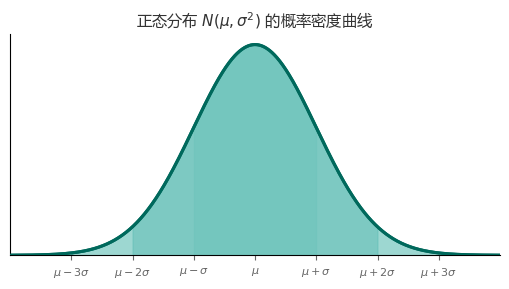
\includegraphics[width=0.62\textwidth]{figs/normal_curve.png}
\end{center}
\[
X\sim N(0,1),\quad
\varphi(x)=\frac1{\sqrt{2\pi}}e^{-\frac{x^{2}}2},\qquad
\Phi(x)=\int_{-\infty}^{x}\varphi(t)\mathrm dt
\]
\[
\bx{\Phi(-x)=1-\Phi(x)},\qquad
\Phi(0)=\frac12
\]
\[
\bx{X\sim N(\mu,\sigma^{2})\Rightarrow Z=\frac{X-\mu}{\sigma}\sim N(0,1)}
\]
\[
\bx{X\sim N(\mu,\sigma^{2})\Rightarrow aX+b\sim N(a\mu+b,\ a^{2}\sigma^{2})}\qquad(a\ne0)
\]
\[
\bx{X,Y\ \text{相互独立},\ X\sim N(\mu_{1},\sigma_{1}^{2}),\ Y\sim N(\mu_{2},\sigma_{2}^{2})
\ \Rightarrow\ X\pm Y\sim N(\mu_{1}\pm\mu_{2},\ \sigma_{1}^{2}+\sigma_{2}^{2})}
\]
\end{formbox}

\hd{随机变量函数的分布}
\begin{formbox}
\[
Y=g(X):\ F_{Y}(y)=P\{g(X)\le y\}=\int_{g(x)\le y}f_{X}(x)\,\mathrm dx
\]
\[
\text{公式法（}\ g\ \text{严格单调可导）：}\quad
f_{Y}(y)=f_{X}\bigl[h(y)\bigr]\bigl|h'(y)\bigr|,\quad h=g^{-1}
\]
\end{formbox}
\end{secbox}

% ============================================================
\begin{secbox}[三、多维随机变量及其分布]

\hd{联合分布、边缘分布与独立性}
\begin{formbox}
\[
F(x,y)=P\{X\le x,\ Y\le y\}
\]
\[
\begin{aligned}
\text{离散：}&
P\{X=x_{i},Y=y_{j}\}=p_{ij};\quad
\text{边缘}\ P\{X=x_{i}\}=\sum_{j}p_{ij}=p_{i\cdot}\\[3pt]
\text{连续：}&
f_{X}(x)=\int_{-\infty}^{+\infty}f(x,y)\,\mathrm dy,
\qquad
f_{Y}(y)=\int_{-\infty}^{+\infty}f(x,y)\,\mathrm dx
\end{aligned}
\]
\[
\bx{X,Y\ \text{独立}\iff F(x,y)=F_{X}(x)F_{Y}(y)
\iff f(x,y)=f_{X}(x)f_{Y}(y)\ \text{（几乎处处）}}
\]
\end{formbox}

\hd{条件分布}
\begin{formbox}
\[
\text{离散：}\quad P\{Y=y_{j}\mid X=x_{i}\}=\frac{p_{ij}}{p_{i\cdot}}
\]
\[
\text{连续：}\quad
f_{Y\mid X}(y\mid x)=\frac{f(x,y)}{f_{X}(x)}\ \ (f_{X}(x)>0)
\]
\end{formbox}

\hd{二维均匀分布与二维正态分布}
\begin{formbox}
\[
(X,Y)\sim U(D):\quad f(x,y)=\begin{cases}\dfrac1{S_{D}},&(x,y)\in D\\[4pt]0,&\text{其他}\end{cases}\quad(S_{D}\ \text{为}\ D\ \text{面积})
\]
\[
(X,Y)\sim N(\mu_{1},\mu_{2};\sigma_{1}^{2},\sigma_{2}^{2};\rho),
\qquad
f(x,y)=\frac1{2\pi\sigma_{1}\sigma_{2}\sqrt{1-\rho^{2}}}\,e^{-\frac12\,Q}
\]
\[
Q=\frac1{1-\rho^{2}}\Bigl[
\frac{(x-\mu_{1})^{2}}{\sigma_{1}^{2}}
-2\rho\frac{(x-\mu_{1})(y-\mu_{2})}{\sigma_{1}\sigma_{2}}
+\frac{(y-\mu_{2})^{2}}{\sigma_{2}^{2}}\Bigr]
\]
\[
(X,Y)\sim N\Rightarrow X\sim N(\mu_{1},\sigma_{1}^{2}),\ Y\sim N(\mu_{2},\sigma_{2}^{2})
\]
\[
\bx{(X,Y)\ \text{为二维正态：}\ X,Y\ \text{独立}\iff X,Y\ \text{不相关}\iff\rho=0}
\]
\end{formbox}

\hd{二维随机变量函数的分布}
\begin{formbox}
\[
Z=X+Y:\quad
f_{Z}(z)=\int_{-\infty}^{+\infty}f(x,z-x)\,\mathrm dx
=\int_{-\infty}^{+\infty}f(z-y,y)\,\mathrm dy
\]
\[
\text{离散：}\quad P\{Z=z\}=\sum_{x}P\{X=x,Y=z-x\}
\]
\[
\bx{M=\max(X,Y):\quad F_{M}(z)=F_{X}(z)F_{Y}(z)}\qquad\text{（独立时）}
\]
\[
\bx{N=\min(X,Y):\quad F_{N}(z)=1-\bigl[1-F_{X}(z)\bigr]\bigl[1-F_{Y}(z)\bigr]}\qquad\text{（独立时）}
\]
\[
X\sim B(n_{1},p),Y\sim B(n_{2},p)\ \text{独立}\Rightarrow X+Y\sim B(n_{1}+n_{2},p)
\]
\end{formbox}
\end{secbox}

% ============================================================
\begin{secbox}[四、随机变量的数字特征]

\hd{数学期望}
\begin{formbox}
\[
\begin{array}{ll}
\text{离散：}\ EX=\displaystyle\sum_{i}x_{i}p_{i}
& \text{连续：}\ EX=\displaystyle\int_{-\infty}^{+\infty}xf(x)\mathrm dx\\[8pt]
E[g(X)]=\displaystyle\sum_{i}g(x_{i})p_{i}
& E[g(X)]=\displaystyle\int_{-\infty}^{+\infty}g(x)f(x)\mathrm dx
\end{array}
\]
\[
E[g(X,Y)]=\iint_{\mathbb R^{2}}g(x,y)f(x,y)\,\mathrm dx\,\mathrm dy
\]
\end{formbox}

\hd{期望与方差的性质}
\begin{formbox}
\[
\begin{aligned}
&E(c)=c, & E(cX)&=c\,EX, & E(X\pm Y)&=EX\pm EY,\\[3pt]
&X,Y\ \text{独立}\Rightarrow E(XY)=EX\cdot EY.
\end{aligned}
\]
\[
\bx{D(X)=E\bigl[(X-EX)^{2}\bigr]=EX^{2}-(EX)^{2}}
\]
\[
\begin{aligned}
&D(c)=0, & D(X+c)&=DX, & D(cX)&=c^{2}DX,\\[3pt]
&X,Y\ \text{独立}\Rightarrow D(X\pm Y)=DX+DY.
\end{aligned}
\]
\[
\bx{DX=0\iff P\{X=c\}=1}
\]
\end{formbox}

\hd{协方差与相关系数}
\begin{formbox}
\[
\bx{\operatorname{Cov}(X,Y)=E\bigl[(X-EX)(Y-EY)\bigr]=E(XY)-EX\cdot EY}
\]
\[
\begin{aligned}
&\operatorname{Cov}(aX,bY)=ab\,\operatorname{Cov}(X,Y),\\[3pt]
&\operatorname{Cov}(X_{1}+X_{2},Y)=\operatorname{Cov}(X_{1},Y)+\operatorname{Cov}(X_{2},Y),\\[3pt]
&D(X\pm Y)=DX+DY\pm2\operatorname{Cov}(X,Y).
\end{aligned}
\]
\[
\bx{\rho_{XY}=\frac{\operatorname{Cov}(X,Y)}{\sqrt{DX}\sqrt{DY}}},\qquad
|\rho_{XY}|\le1
\]
\[
\bx{\text{不相关}\iff \operatorname{Cov}(X,Y)=0\iff E(XY)=EX\cdot EY\iff D(X+Y)=DX+DY\iff\rho=0}
\]
\[
|\rho|=1\iff P\{Y=aX+b\}=1\ \ (a\ne0)
\]
\[
\bx{\text{独立}\Rightarrow\text{不相关};\qquad \text{不相关}\nRightarrow\text{独立}}
\]
\[
\text{二维正态：独立}\iff\text{不相关};\qquad
X\sim B(1,p),Y\sim B(1,p):\text{独立}\iff\text{不相关}
\]
\end{formbox}

\hd{矩}
\begin{formbox}
\[
\text{$k$ 阶原点矩}\ E(X^{k});\qquad
\text{$k$ 阶中心矩}\ E\bigl[(X-EX)^{k}\bigr]
\]
\[
\text{混合原点矩}\ E(X^{k}Y^{l});\qquad
\text{混合中心矩}\ E\bigl[(X-EX)^{k}(Y-EY)^{l}\bigr]
\]
\end{formbox}

\hd{常见分布期望方差汇总}
\begin{formbox}
\begin{center}
\renewcommand{\arraystretch}{1.5}
\begin{tabular}{|c|c|c|c|}
\hline
分布 & 参数 & $E(X)$ & $D(X)$ \\ \hline
0-1 分布 $B(1,p)$ & $0<p<1$ & $p$ & $p(1-p)$ \\ \hline
二项 $B(n,p)$ & $n,p$ & $np$ & $np(1-p)$ \\ \hline
几何 $G(p)$ & $0<p<1$ & $\dfrac1p$ & $\dfrac{1-p}{p^{2}}$ \\ \hline
泊松 $P(\lambda)$ & $\lambda>0$ & $\lambda$ & $\lambda$ \\ \hline
均匀 $U(a,b)$ & $a<b$ & $\dfrac{a+b}{2}$ & $\dfrac{(b-a)^{2}}{12}$ \\ \hline
指数 $E(\lambda)$ & $\lambda>0$ & $\dfrac1\lambda$ & $\dfrac1{\lambda^{2}}$ \\ \hline
正态 $N(\mu,\sigma^{2})$ & $\mu,\sigma^{2}$ & $\mu$ & $\sigma^{2}$ \\ \hline
\end{tabular}
\end{center}
\end{formbox}
\end{secbox}

% ============================================================
\begin{secbox}[五、大数定律与中心极限定理]

\hd{切比雪夫不等式}
\begin{formbox}
\[
\bx{\forall\varepsilon>0,\quad P\bigl\{|X-EX|\ge\varepsilon\bigr\}\le\frac{DX}{\varepsilon^{2}}}
\]
\[
P\bigl\{|X-EX|<\varepsilon\bigr\}\ge1-\frac{DX}{\varepsilon^{2}}
\]
\end{formbox}

\hd{大数定律}
\begin{formbox}
\hd{切比雪夫大数定律}
\[
X_{1},\dots,X_{n}\ \text{相互独立},\ DX_{i}\ \text{一致有上界}\Rightarrow
\lim_{n\to\infty}P\Bigl\{\Bigl|\frac1n\sum_{i=1}^{n}X_{i}-\frac1n\sum_{i=1}^{n}EX_{i}\Bigr|<\varepsilon\Bigr\}=1
\]
\hd{辛钦大数定律}
\[
X_{1},\dots,X_{n}\ \text{独立同分布},\ EX_{i}=\mu\Rightarrow
\lim_{n\to\infty}P\Bigl\{\Bigl|\frac1n\sum_{i=1}^{n}X_{i}-\mu\Bigr|<\varepsilon\Bigr\}=1
\]
\hd{伯努利大数定律}
\[
X\sim B(n,p)\Rightarrow
\lim_{n\to\infty}P\Bigl\{\Bigl|\frac Xn-p\Bigr|<\varepsilon\Bigr\}=1
\]
\end{formbox}

\hd{中心极限定理}
\begin{formbox}
\hd{列维—林德伯格中心极限定理}
\[
X_{1},\dots,X_{n}\ \text{独立同分布},\ EX_{i}=\mu,\ DX_{i}=\sigma^{2}\Rightarrow
\lim_{n\to\infty}P\Bigl\{\frac{\sum X_{i}-n\mu}{\sqrt n\,\sigma}\le x\Bigr\}=\Phi(x)
\]
\hd{棣莫弗—拉普拉斯中心极限定理}
\[
X\sim B(n,p)\Rightarrow
\lim_{n\to\infty}P\Bigl\{\frac{X-np}{\sqrt{np(1-p)}}\le x\Bigr\}=\Phi(x)
\]
\end{formbox}
\end{secbox}

% ============================================================
\begin{secbox}[六、数理统计]

\hd{总体、样本与统计量}
\begin{formbox}
\[
\bar X=\frac1n\sum_{i=1}^{n}X_{i},\qquad
S^{2}=\frac1{n-1}\sum_{i=1}^{n}(X_{i}-\bar X)^{2}
\]
\[
\text{样本}\ k\ \text{阶原点矩}\ A_{k}=\frac1n\sum_{i=1}^{n}X_{i}^{k};\qquad
\text{样本}\ k\ \text{阶中心矩}\ B_{k}=\frac1n\sum_{i=1}^{n}(X_{i}-\bar X)^{k}
\]
\[
E\bar X=\mu,\qquad D\bar X=\frac{\sigma^{2}}{n},\qquad ES^{2}=\sigma^{2}
\]
\end{formbox}

\hd{三大抽样分布}
\begin{formbox}
\[
\bx{\chi^{2}\sim\chi^{2}(n):\quad \chi^{2}=X_{1}^{2}+\cdots+X_{n}^{2},\ X_{i}\overset{\text{iid}}{\sim}N(0,1)},\quad
E(\chi^{2})=n,\ D(\chi^{2})=2n
\]
\[
\chi_{1}^{2}\sim\chi^{2}(n_{1}),\ \chi_{2}^{2}\sim\chi^{2}(n_{2})\ \text{独立}\Rightarrow
\chi_{1}^{2}+\chi_{2}^{2}\sim\chi^{2}(n_{1}+n_{2})
\]
\[
\bx{t\sim t(n):\quad t=\frac{X}{\sqrt{Y/n}},\ X\sim N(0,1),\ Y\sim\chi^{2}(n),\ X,Y\ \text{独立}}
\]
\[
t_{1-\alpha}(n)=-t_{\alpha}(n),\qquad\text{密度为偶函数，}\ n\to\infty\ \text{时}\ t(n)\to N(0,1)
\]
\[
\bx{F\sim F(n_{1},n_{2}):\quad F=\frac{X/n_{1}}{Y/n_{2}},\ X\sim\chi^{2}(n_{1}),\ Y\sim\chi^{2}(n_{2})\ \text{独立}}
\]
\[
\bx{F_{1-\alpha}(n_{1},n_{2})=\frac1{F_{\alpha}(n_{2},n_{1})}},\qquad
\frac1F\sim F(n_{2},n_{1})
\]
\end{formbox}

\hd{正态总体的抽样分布}
\begin{formbox}
$X_{1},\dots,X_{n}$ 为来自 $N(\mu,\sigma^{2})$ 的样本：
\[
\bx{\bar X\sim N\Bigl(\mu,\frac{\sigma^{2}}n\Bigr)},\qquad
\bx{\frac{\bar X-\mu}{\sigma/\sqrt n}\sim N(0,1)}
\]
\[
\bx{\frac{(n-1)S^{2}}{\sigma^{2}}\sim\chi^{2}(n-1)},\qquad
\bx{\frac{\bar X-\mu}{S/\sqrt n}\sim t(n-1)},\qquad
\bar X\ \text{与}\ S^{2}\ \text{相互独立}
\]
\end{formbox}

\hd{参数估计}
\begin{formbox}
\hd{矩估计}（令样本矩 $=$ 总体矩，解出未知参数）：
\[
E(X^{k})=\frac1n\sum_{i=1}^{n}X_{i}^{k}
\]
\hd{极大似然估计}：
\[
L(\theta)=\prod_{i=1}^{n}f(x_{i};\theta)\quad\text{或}\quad\prod_{i=1}^{n}P\{X=x_{i};\theta\},
\qquad
\frac{\mathrm d\ln L}{\mathrm d\theta}=0\Rightarrow\hat\theta
\]
\end{formbox}

\hd{区间估计（置信水平 $1-\alpha$）}
\begin{formbox}
\[
\sigma^{2}\ \text{已知}:\ \mu\ \text{置信区间}\quad
\Bigl(\bar X-\frac{\sigma}{\sqrt n}z_{\alpha/2},\ \bar X+\frac{\sigma}{\sqrt n}z_{\alpha/2}\Bigr)
\]
\[
\sigma^{2}\ \text{未知}:\ \mu\ \text{置信区间}\quad
\Bigl(\bar X-\frac{S}{\sqrt n}t_{\alpha/2}(n-1),\ \bar X+\frac{S}{\sqrt n}t_{\alpha/2}(n-1)\Bigr)
\]
\[
\mu\ \text{未知}:\ \sigma^{2}\ \text{置信区间}\quad
\Bigl(\frac{(n-1)S^{2}}{\chi^{2}_{\alpha/2}(n-1)},\ \frac{(n-1)S^{2}}{\chi^{2}_{1-\alpha/2}(n-1)}\Bigr)
\]
\end{formbox}

\hd{单个正态总体的假设检验}
\begin{formbox}
\begin{center}
\renewcommand{\arraystretch}{1.6}
\begin{tabular}{|c|c|c|c|c|}
\hline
原假设 $H_{0}$ & 备择 $H_{1}$ & 条件 & 检验统计量 & 拒绝域 \\ \hline
$\mu=\mu_{0}$ & $\mu\ne\mu_{0}$ & $\sigma^{2}$ 已知 & $Z=\dfrac{\bar X-\mu_{0}}{\sigma/\sqrt n}$ & $|Z|\ge z_{\alpha/2}$ \\ \hline
$\mu\le\mu_{0}$ & $\mu>\mu_{0}$ & $\sigma^{2}$ 已知 & $Z=\dfrac{\bar X-\mu_{0}}{\sigma/\sqrt n}$ & $Z\ge z_{\alpha}$ \\ \hline
$\mu\ge\mu_{0}$ & $\mu<\mu_{0}$ & $\sigma^{2}$ 已知 & $Z=\dfrac{\bar X-\mu_{0}}{\sigma/\sqrt n}$ & $Z\le -z_{\alpha}$ \\ \hline
$\mu=\mu_{0}$ & $\mu\ne\mu_{0}$ & $\sigma^{2}$ 未知 & $t=\dfrac{\bar X-\mu_{0}}{S/\sqrt n}$ & $|t|\ge t_{\alpha/2}(n-1)$ \\ \hline
$\mu\le\mu_{0}$ & $\mu>\mu_{0}$ & $\sigma^{2}$ 未知 & $t=\dfrac{\bar X-\mu_{0}}{S/\sqrt n}$ & $t\ge t_{\alpha}(n-1)$ \\ \hline
$\mu\ge\mu_{0}$ & $\mu<\mu_{0}$ & $\sigma^{2}$ 未知 & $t=\dfrac{\bar X-\mu_{0}}{S/\sqrt n}$ & $t\le -t_{\alpha}(n-1)$ \\ \hline
$\sigma^{2}=\sigma_{0}^{2}$ & $\sigma^{2}\ne\sigma_{0}^{2}$ & $\mu$ 未知 & $\chi^{2}=\dfrac{(n-1)S^{2}}{\sigma_{0}^{2}}$ & $\chi^{2}\le\chi^{2}_{1-\alpha/2}$ 或 $\chi^{2}\ge\chi^{2}_{\alpha/2}$ \\ \hline
\end{tabular}
\end{center}

两类错误：
\[
\bx{\alpha=P\{\text{拒绝}\ H_{0}\mid H_{0}\ \text{为真}\}}\quad\text{（第一类错误、弃真）}
\]
\[
\bx{\beta=P\{\text{接受}\ H_{0}\mid H_{0}\ \text{为假}\}}\quad\text{（第二类错误、取伪）}
\]
\end{formbox}
\end{secbox}

\end{document}